\chapter{Systematic uncertainties}
\label{sec:Lb_sys}

\section{Yields}
\label{sec:Lb_yield_sys}

The choice of a specific PDF to model the invariant mass distribution coule result
in a bias. In order to asses the effect of the signal PDF choice a number of models
are tried on the \Lb\to\jpsi\Lz data sample in order to understand which ones are plausible.
In Tab.~\ref{PDFsys} are reported the $\chi^2$ relative probabilities obtained using different
models including: the default model, a Double Crystal Ball function, a simple Gaussian function,
a simple Crystal Ball function and the sum of two Gaussians. The only two models that
give a reasonable p-value are the default DCB and the sum of two Gaussian functions (DG).
As a second step simulated experiments are generated and fit the two chosen functions.
Events are generated according to a density function given by the default model fitted
on data separately for each \qsq interval. In this way, for each \qsq interval, a specific
shape is reproduced including the background level and slope. Furthermore, a number 
of events comparable to the one found in data is generated. For each experiment a per cent bias
is calculated as
%
\begin{equation}
b = \left(\frac{N^{DCB}_{\ell\ell}}{N^{DCB}_{\jpsi}} - \frac{N^{DG}_{\ell\ell}}{N^{DG}_{\jpsi}}\right) / \frac{N^{DCB}_{\ell\ell}}{N^{DCB}_{\jpsi}}
\end{equation}
%
where $N^{model}_{\ell\ell}$ and $N^{model}_{\jpsi}$ are the numbers of rare and resonant events
observed using a specific model. The distribution of biases have approximately gaussian shape.
Finally, the average bias over 1000 pseudo-experiments is taken
as systematic uncertainty. Notice that in each case the rare and normalisation channels are fit
with the same signal model and, while for the default case the rare parameters are fixed to what found
for the resonant channel, they are left free to float with the second model in order to asses
at the same time the systematic due to the parameters contraint.

\begin{center}
\begin{table}[h]
\centering
\caption{$\chi^2$, NDF, p-values and number of signal events obtained fitting \Lb\to\jpsi\Lz data using different models.}
\begin{tabular}{lcccc}
\hline
Model   		& $\chi^2/NDF$  & $NDF$  & p-value  & $N_{evts}$ \\ \hline
%\multicolumn{4}{c}{Rare channel} \\
%DCB  (default)  &    1.1   &   47   &    0.34       &  279.8  \\
%Gauss 		&    1.0   &   46   &    0.55       &  270.3  \\
%Double gauss  	&    1.0   &   44   &    0.47       &  270.3  \\
%CB  		&    1.0   &   44   &    0.47       &  270.4  \\
%\hline
%$K_S$ removed 	&    1.0   &   47   &    0.41       &  283.5  \\
%\hline
%\multicolumn{4}{c}{$J/\psi$ channel} \\
%\hline
DCB  (default)	&    1.0   &   187   &    0.51      & 9965.4  \\
Gauss			&    1.8   &   193   &    $\sim 0$  & 9615.7 \\
Double Gauss  	&    1.1   &   191   &    0.45      & 9882.4  \\
CB  			&    1.5   &   191   &    $\sim 0$  & 9802.4 \\
%\hline
%Fixed $K_S$ shape &  1.6   &   188   &    $\sim 0$  & 9976.3  \\
%With $K^{*0}$ bkg &    1.0   &   188   &    0.53      & 9976.4  \\
\hline
\end{tabular}
\label{PDFsys}
\end{table}
\end{center}

For the background PDF systematic the rare channel is refit leaving the yield of \KS component floating,
which is fixed to the predicted value in the default fit. The same procedure as for the signal PDF is applied.
Results are reported in Tab.~\ref{tab:pdfsys}. The most affected bin is the one in the middle of the charmonium
resonances, where a combination of lower statistics and higher background leaves more freedom to the signal shape.
Finally, a background component for $B^{+} \ra K^{*+}(\KS\pi^+)\mumu$ decays is added in the fit, modelled using
the distribution of simulated events after full selection. No significant bias is found for this component.

\begin{center}
\begin{table}[h]
\centering
\begin{tabular}{lccc}
\hline
\qsq [\gevgevcccc] & Sig. PDF bias (\%)  & Bkg. PDF bias (\%)  & Tot. sys. (\%) \\ \hline
0.1--2.0       &    3.2   &  1.1   &    3.4    \\
2.0--4.0       &    2.9   &  2.4   &    3.8    \\
4.0--6.0       &    4.6   &  4.8   &    6.6    \\
6.0--8.0       &    1.2   &  1.7   &    2.0    \\

11.0--12.5		&    2.6   &  1.8   &    3.2	\\
15.0--16.0 	&    1.3   &  2.5   &    2.8	\\
16.0--18.0 	&    0.6   &  1.3   &    1.4	\\
18.0--20.0 	&    1.7   &  1.8   &    2.5	\\

\hline
1.1--6.0       &    0.1   &  4.2   &    4.2    \\
15.0--20.0		&    1.0   &  0.2   &    1.1	\\
\hline
\end{tabular}
\caption{ Values of systematics due to the choice of signal and background shapes in bins of \qsq. }
\label{tab:pdfsys}
\end{table}
\end{center}




\section{Efficiencies}

%As we study \qsq dependence of the differential branching fraction, one of the challenges is to properly account for
%correlations. There are three types of correlations we need to handle, one is correlation between
%normalisation and signal decay, second is correlation between different \qsq bins and finally as we
%split efficiency into three parts (geometry, selection and trigger), we should take also correlation
%amongst them into account. The last class of correlations is in principle rather easy to treat, but
%fully correct treatment of the first two classes would require to split the systematic uncertainties
%to correlated amongst \qsq bins and uncorrelated part, which given our statistics would complicate
%the presentation of the result. For simplicity we treat correlations where systematic uncertainty is
%significant and neglect correlations amongst \qsq bins when uncertainty for given source is small
%compared to dominant sources.
%
Systematic uncertainties in the efficiency determination are due to limited knowledge
of the decay properties such as the \Lb lifetime and production polarisation.
The uncertainties are directly calculated on the relative efficiencies as these are the ones that
are actually used in the analysis. It should be noted that not all sources contribute to each part
of the efficiency. For brevity in this section are only reported estimates of the systematic
uncertainties obtained while the full information is contained in App.~\ref{app:Lb_systematics}.
%Numerical values of systematic uncertainties on relative efficiencies are in
%table \ref{tab:relativeGeomSys} and for \ref{tab:relativeDetSys} for geometrical and detection efficiency;
%\ref{tab:relativeRecoSys}, \ref{tab:relativeTrigSys} and \ref{tab:relativeMVAsys} for reconstruction, trigger and neural
%networks for long-long and down-down events.
%Finally, we remind the reader that we always use fully simulated phase space sample we weight those, modelling
%polarisation and decay structure. The MC sample used is always the same thus within the single decay there is always
%correlation in our simulated events.
%

\subsubsection{Effect of new physics on the decay model}
\label{sec:WCvariation}

New physics could affect the decay model modifying the Wilson Coefficients by adding
contributions to the $C_7$ and $C_9$ coefficients. This would result in a modification
of the \qsq spectrum and therefore of the efficiency.
To asses this systematic Wilson Coefficients are modified by adding a NP component
($C_i \rightarrow C_i + C_i^{ \rm NP}$). In Fig.~\ref{fig:wilson_q2} are reported \qsq spectra
obtained weighting the simulation for a model embedding the default and 3 modified sets
of wilson coefficients. Used values used are reported on top of each plot and are inspired
to maintain compatibility with the recent LHCb result for the $P'_5$ observable~\cite{Descotes-Genon:2013wba}.
The biggest effect is in the very low \qsq, belo 2 \gevgevcccc the efficiency can change
up to 7\%, 3-4 \% between 3 and 4 \gevgevcccc and 2-3 \% in the resto of the spectrum.
This values are given in order to provide the full information but are not added as systematic
uncertainties. In fact the hypothesis of this analysis is that the decays are described
by a the SM.

\begin{figure}
\centering
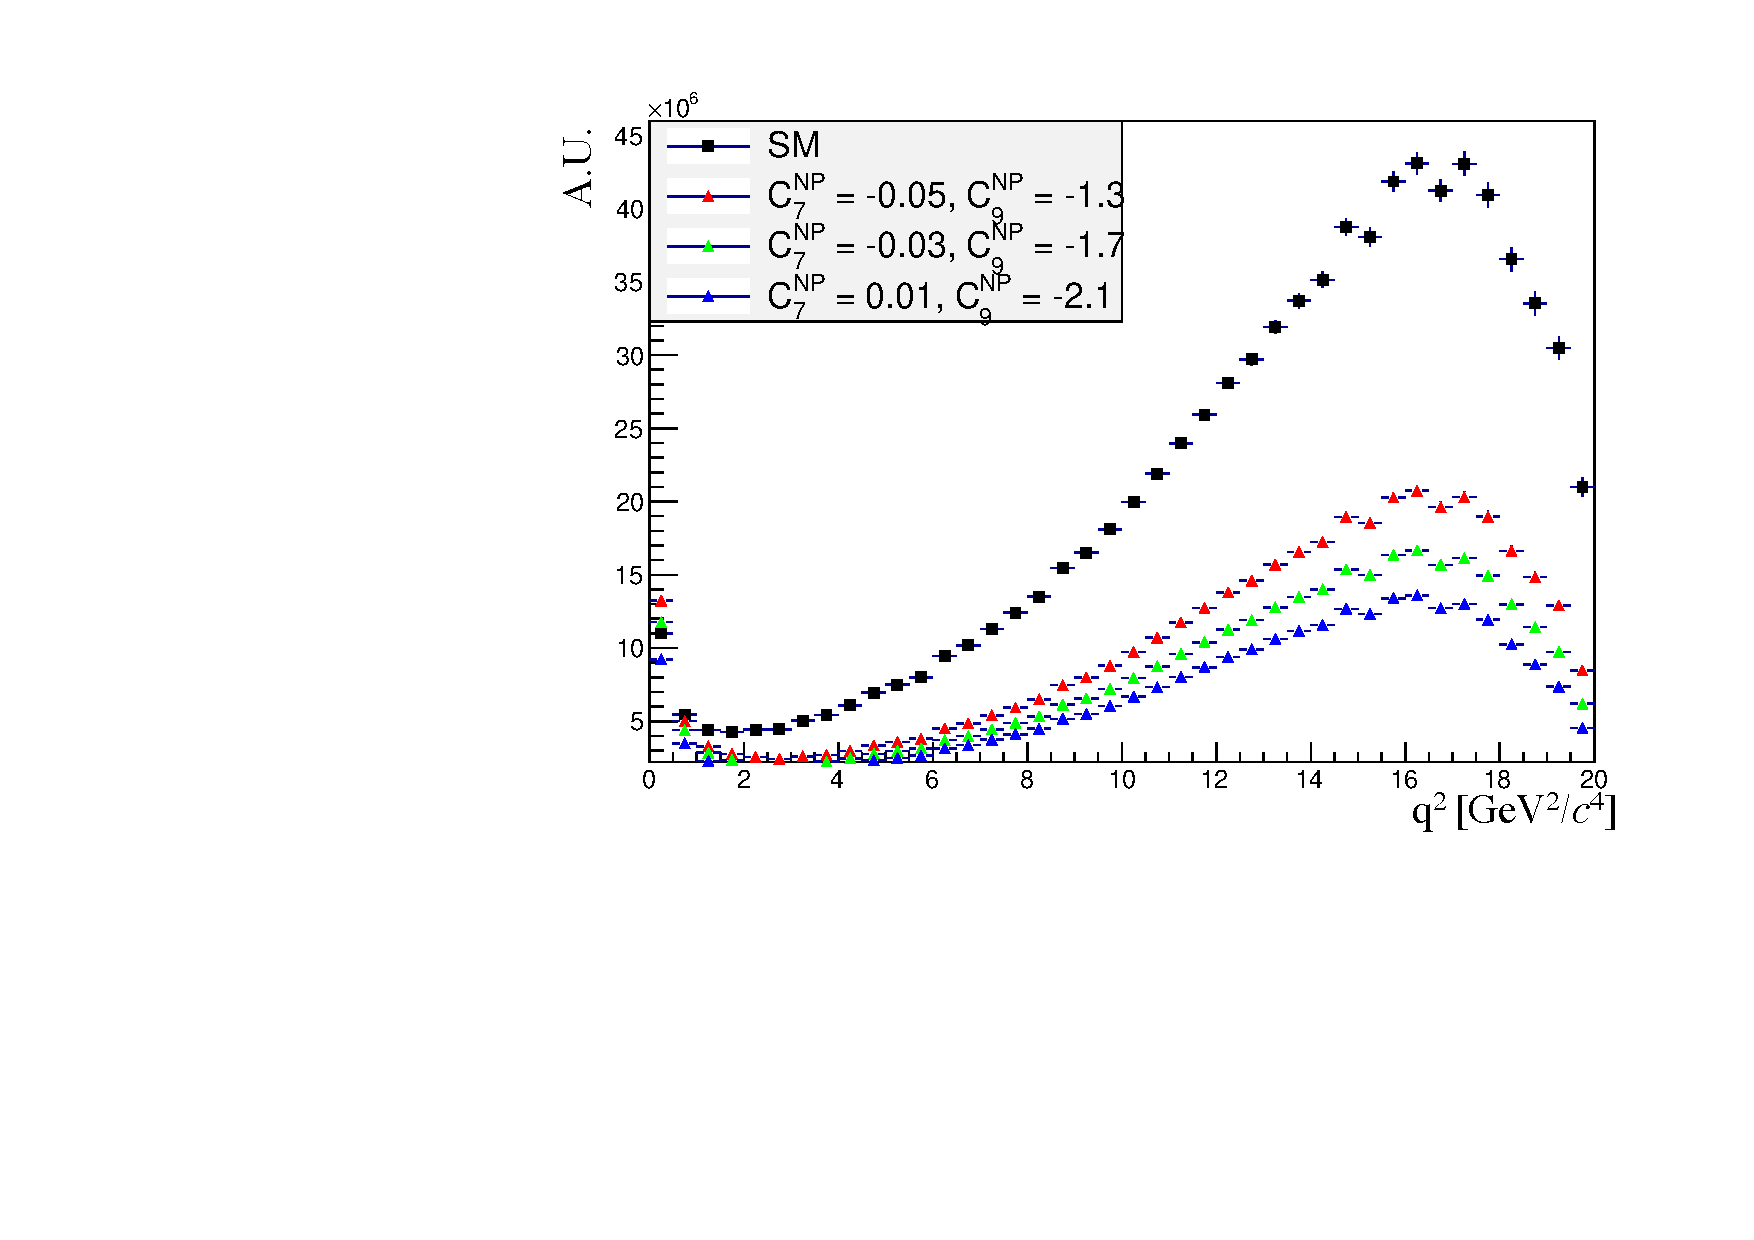
\includegraphics[width=0.8\textwidth]{Lmumu/figs/wilson_q2.pdf}
\caption{The \qsq spectrum of $\Lb\to\Lz\mumu$ events weighted with models embedding different sets of Wilson Coefficients.
The black distribution corresponds to the weighting used to calculate efficiencies.}
\label{fig:wilson_q2}
\end{figure}

%\begin{figure}
%\centering
%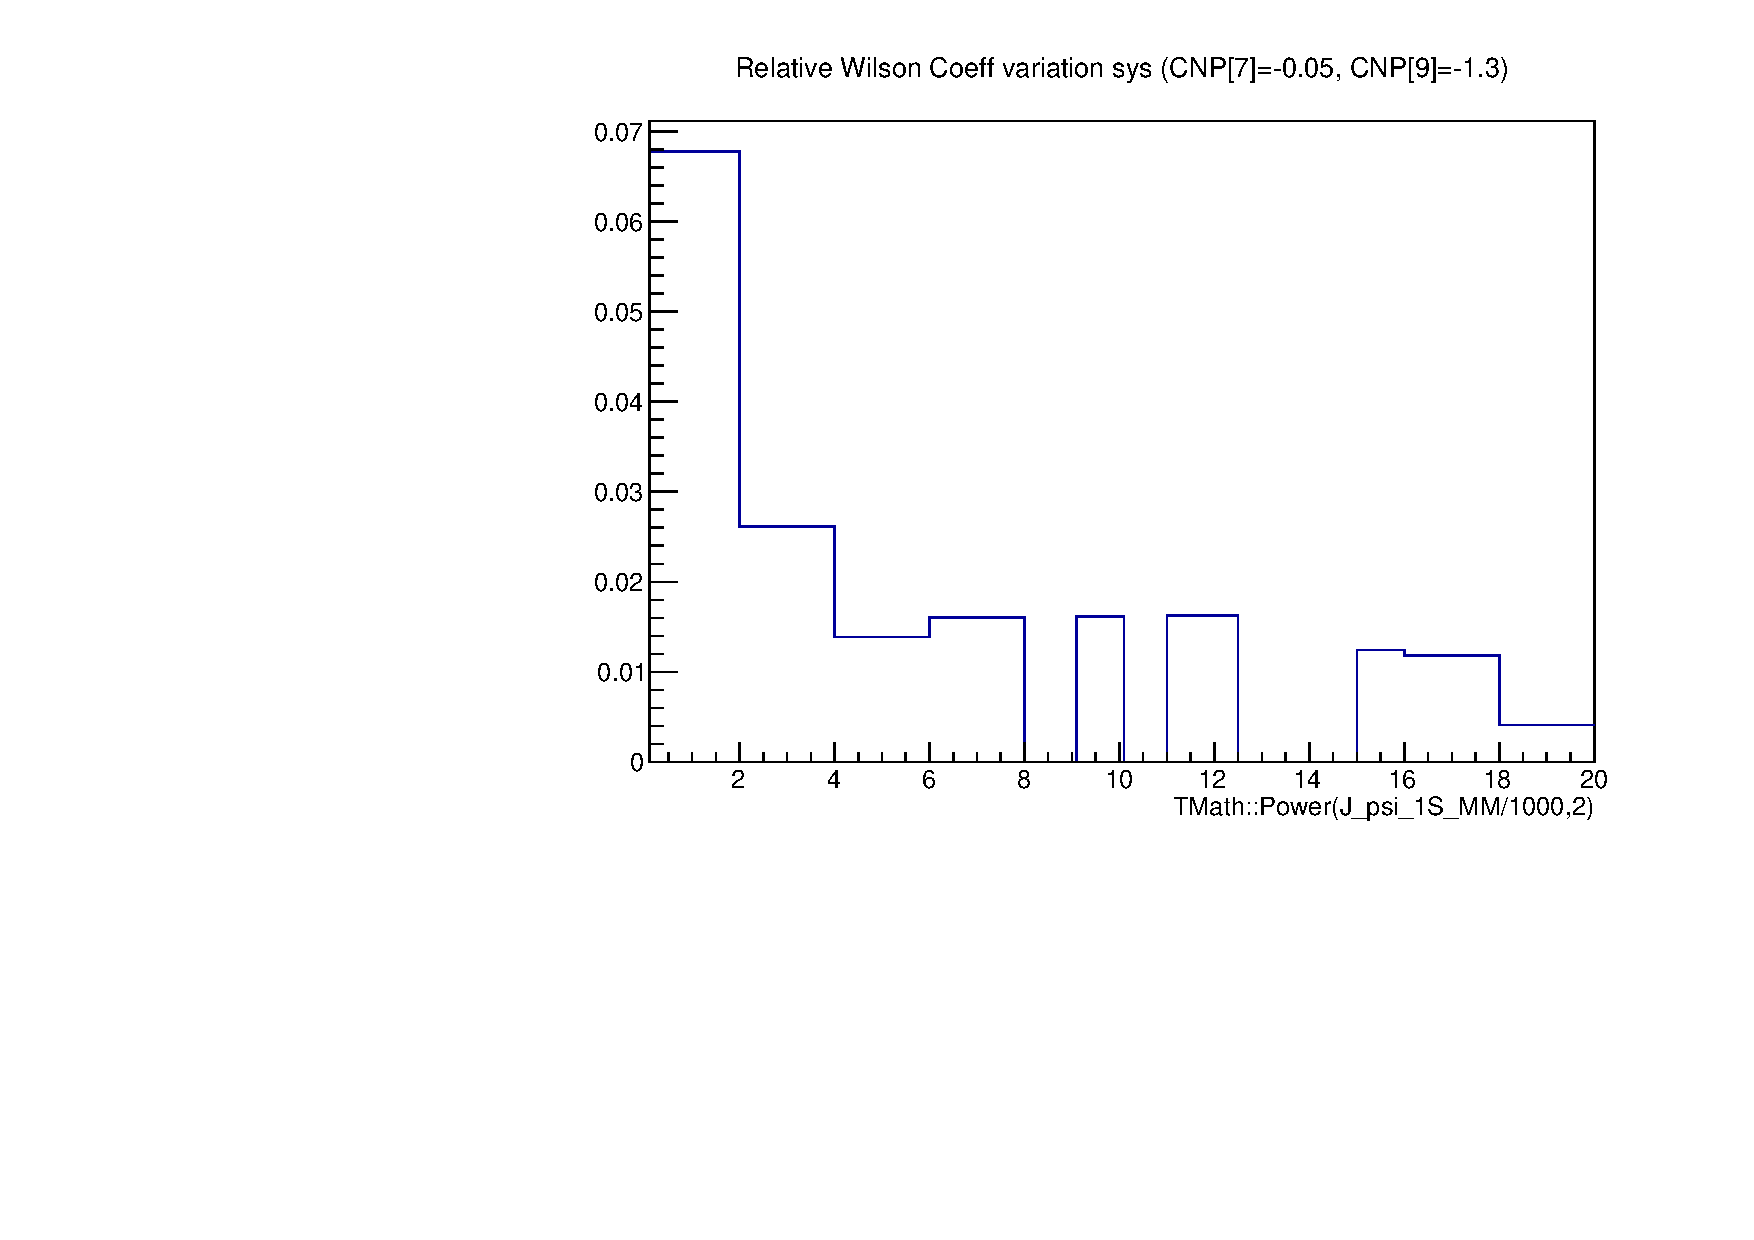
\includegraphics[width=0.48\textwidth]{Lmumu/figs/rel_wilson1_sysAll.pdf}
%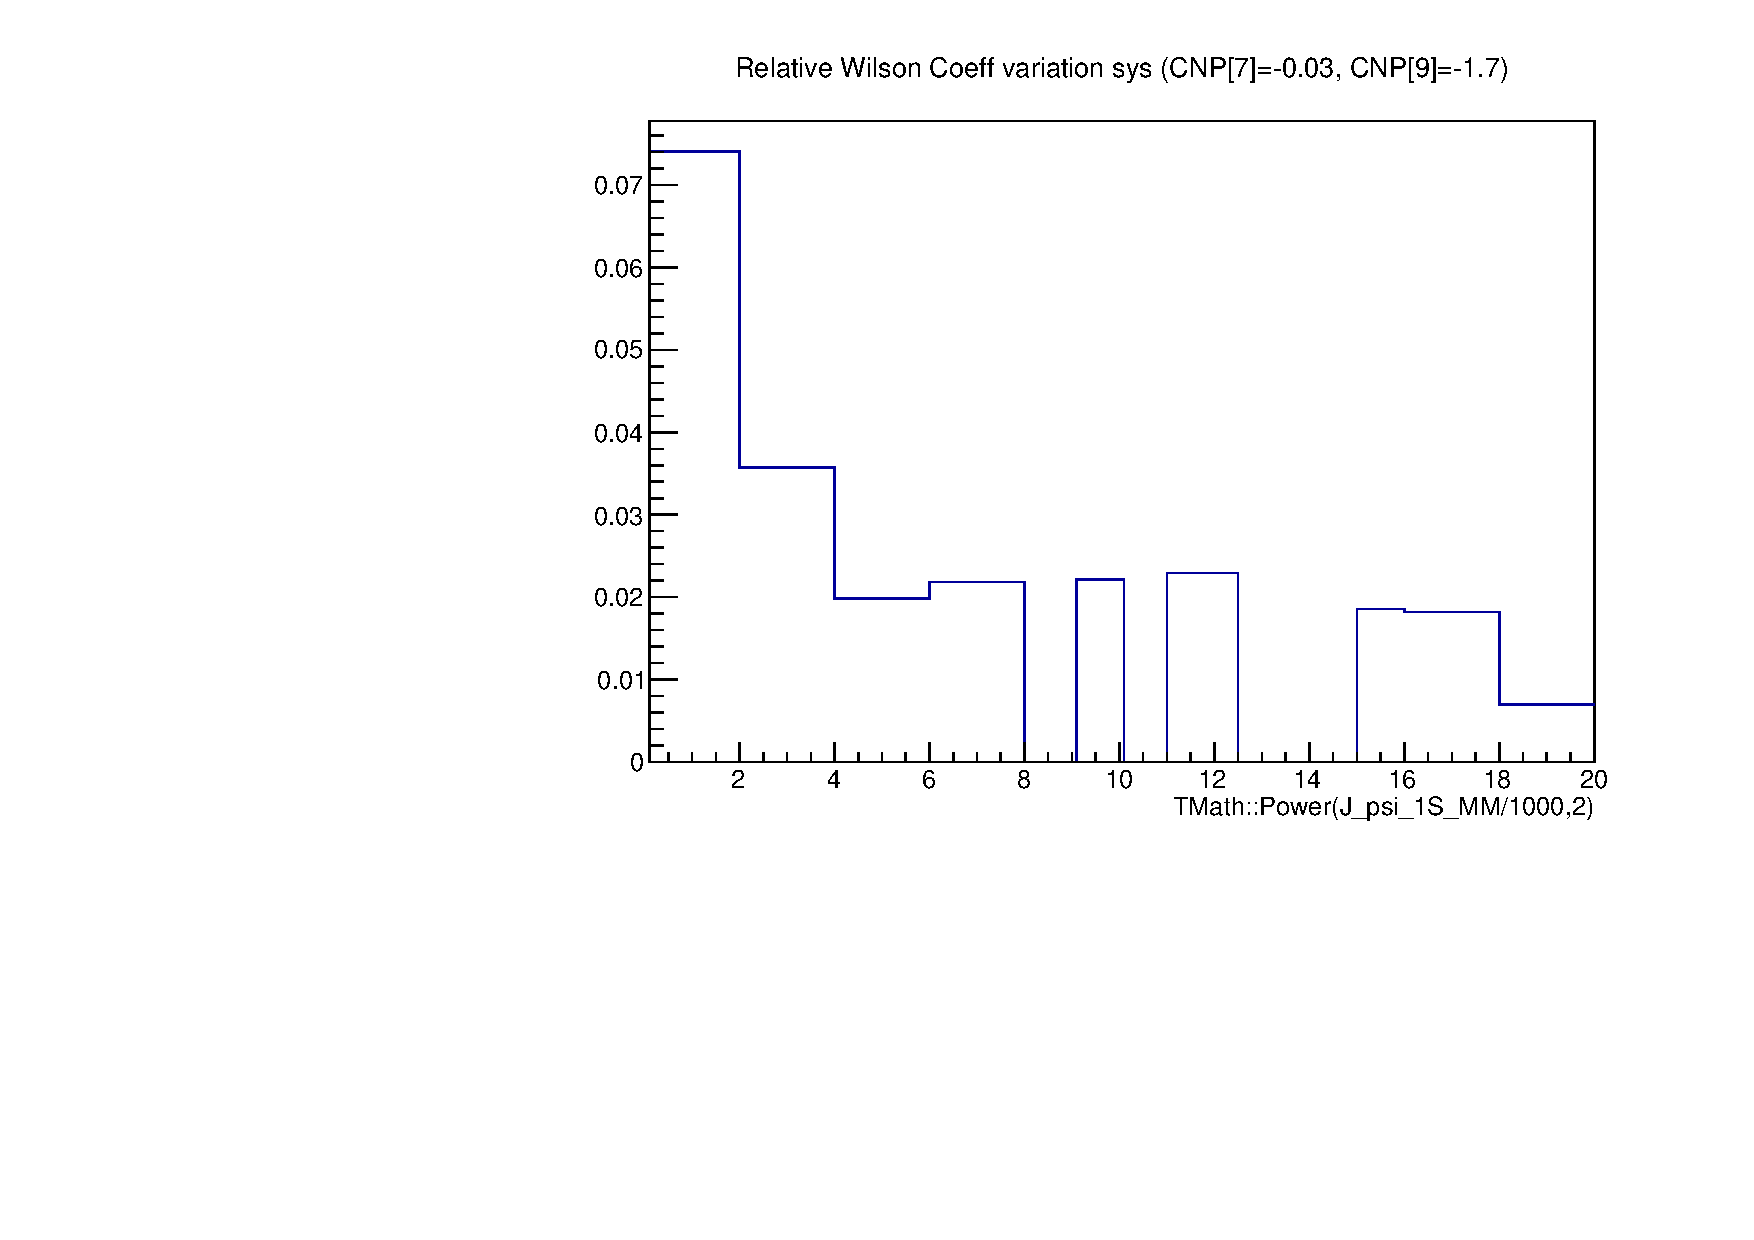
\includegraphics[width=0.48\textwidth]{Lmumu/figs/rel_wilson2_sysAll.pdf} \\
%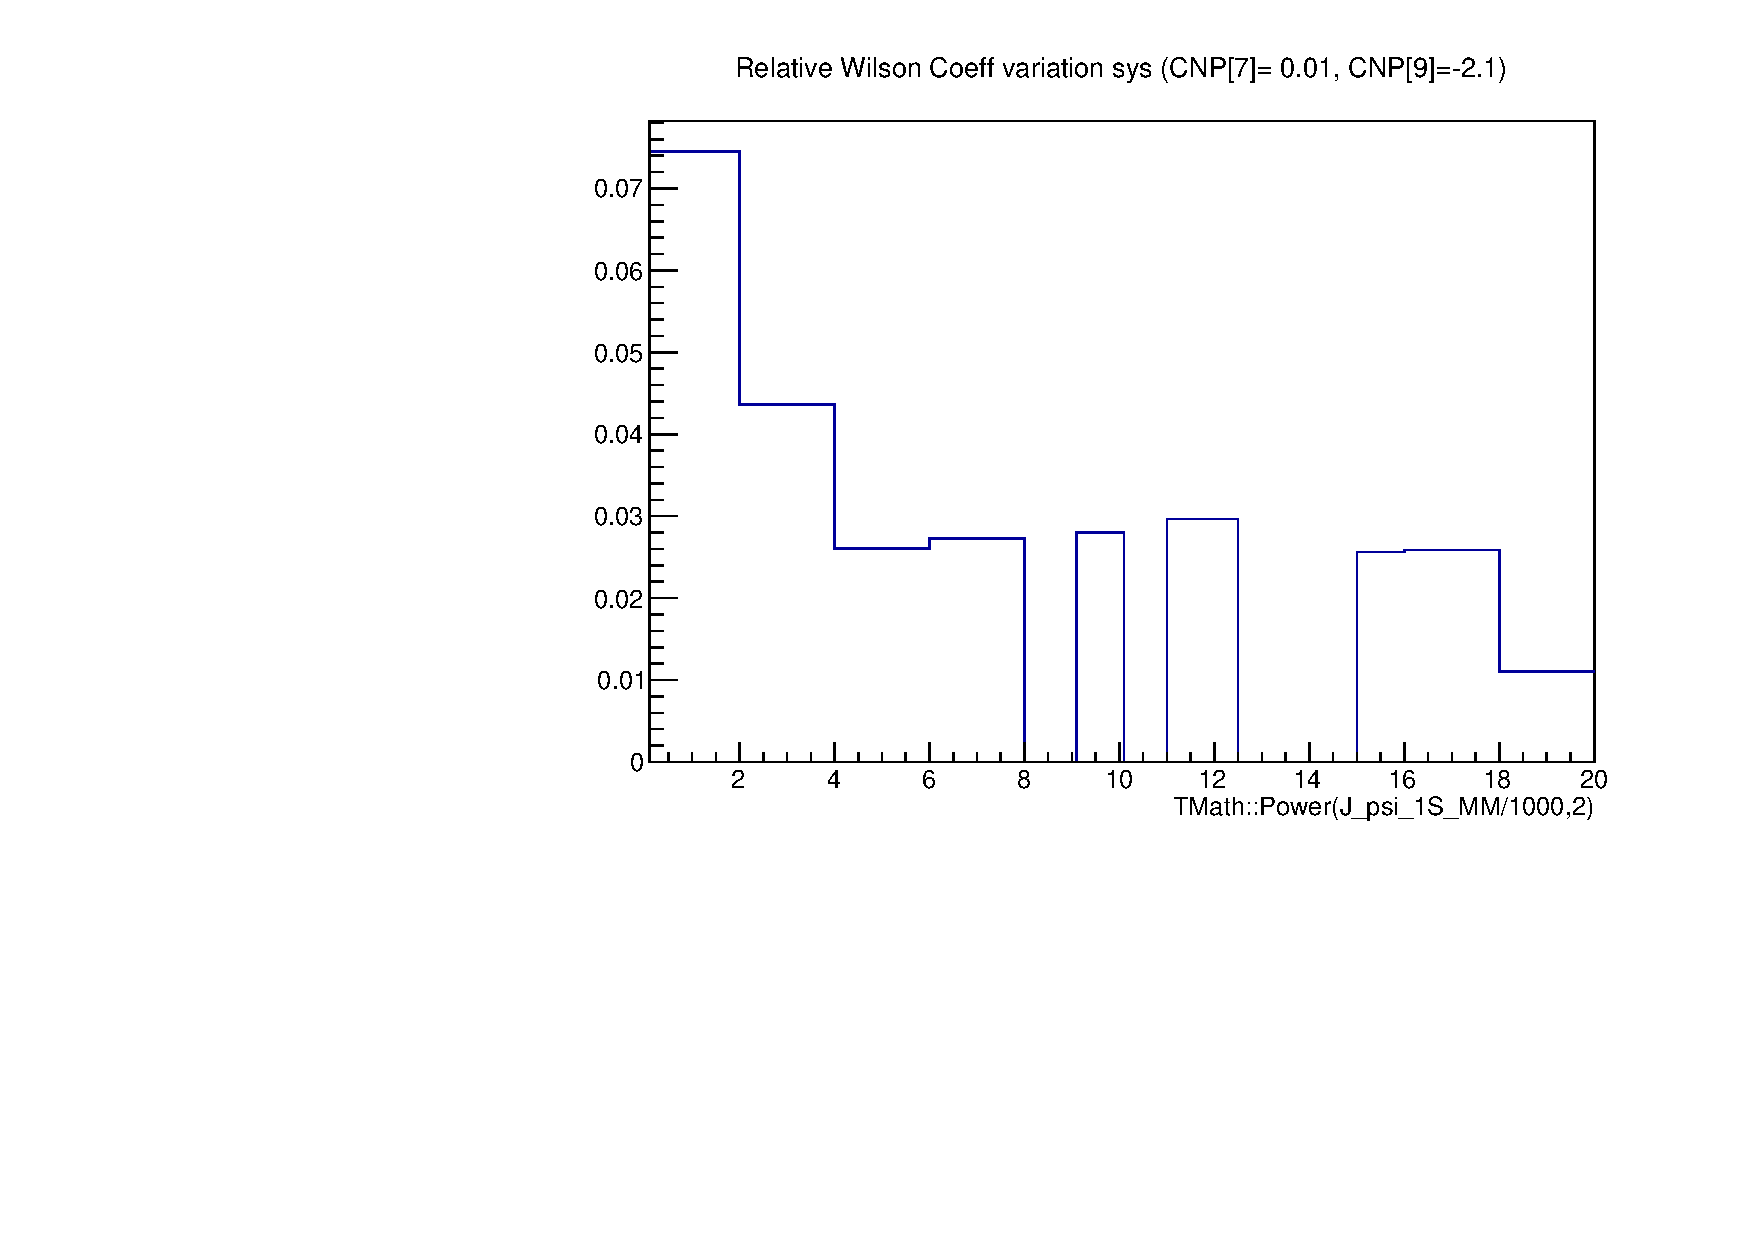
\includegraphics[width=0.48\textwidth]{Lmumu/figs/rel_wilson3_sysAll.pdf}
%\caption{Relative effect of different Wilson Coefficients sets on the total efficiency in bins of \qsq.}
%\label{fig:wilson_diff}
%\end{figure}

\subsection{Simulation statistics}

The limited statistics of the simulated samples used to determine efficiencies is considered a source of systematic uncertainty.
While it is not the dominant source of systematics, its size does not allow to completely neglect this uncertainty.
When reporting relative efficiency values the statistical uncertainty due to the  rare and resonant channels
is always considered. 
%While it would be useful to treat part from normalisation channel separately due to the correlation 
%across \qsq bins, given its size we decide to suppress it as in final presentation its effect is hard to see.

\subsection{Production polarisation and decay structure}
\label{sec:BRpolsys}

One of the main unknown which affects the determination of the efficiencies is the angular structure of
the decays. And connected to it also the production polarisation, which is a parameter of the model.
%The normalisation decay $\Lb\to\jpsi\Lz$ is also re-weighted and $\Lb\to\Lz\mumu$ is
%distributed according to the model described in appendix \ref{ap:LbLmumuAngular}.
%
To assess the systematic uncertainty due to the knowledge of the production polarisation for $\Lb\to\Lz\mumu$ decays
the polarisation parameter in the model is varied within one standard deviation of the
most recent LHCb measurement $P = 0.06 \pm 0.09$\cite{Aaij:2013oxa}. The full difference observed is
taken as systematic uncertainty. To assess systematic uncertainty due to decay structure
an alternative set of form factors is used based on lattice QCD calculation~\cite{Detmold:2012vy}.
Details of this are explained in \ref{ap:LbLmumuAngular}. The two models are compared and the full difference
is taken as systematic uncertainty.
%
In total this results in an uncertainty of $\sim 1.3\%$ for long candidates and $\sim 0.6\%$ for downstream
candidates, mostly coming from the knowledge of the production polarisation.

\subsection{\Lb lifetime}

The \Lb lifetime is known only with limited precision. For evaluation of the efficiencies the
world average value, 1.482 ps$^{-1}$~\cite{Aaij:2013oha} is used. To evaluate the systematic uncertainty,
this values is varied within one standard deviation from the measured value.
Only cases where both signal and normalisation channel are varied in same direction are considered.
The larger difference with the default lifetime case is taken as systematic uncertainty,
which is found to range from $\sim 0.4\%$ at low \qsq to $\sim 0.1\%$ at high \qsq.
%We do not attempt to separate out part correlated amongst \qsq bins. This source does not affect
%geometric acceptance, which is defined purely by requirements on angles of each muon with respect to
%beam axis.

\subsection{Downstream candidates reconstruction efficiency}

%In the LHCb detector, \Lz can be reconstructed using long or downstream tracks. The distinction is mainly
%driven by the geometry of the detector. A potential issue is that fraction of \Lz reconstructed
%from long tracks and downstream tracks does not fully agree with simulation. For $\Lb\to\jpsi\Lz$
%decay we determine on data that $(26.44 \pm 0.70)$\% of \Lz candidates are reconstructed from long tracks.
%On contrary in simulation of the same decay, only $21.15\pm0.24$\% of candidates are reconstructed
%from long tracks. The same ratio on phase space simulation of $\Lb\to\Lz\mumu$ is $21.54\pm0.14$\%
%(integrated over \qsq). From this we conclude that this ratio is expected to be similar in the two samples and
%that simulation does not fully match data.

Other analysis in LHCb, using particles reconstructed with downstream tracks, showed that
the efficiency for these events is not well simulated in the Monte Carlo.
For example in Fig.~\ref{KS_vtxeff} the ratio between the reconstruction efficiency for downstream candidates
in data and simulation found analysing \KS events~\cite{Blake:1631348} is shown. This effect is not
yet fully understood and is currently under study. The main effect seems to be due to a poor simulation
of the vertexing efficiency for downstream tracks.

\begin{figure}
\centering
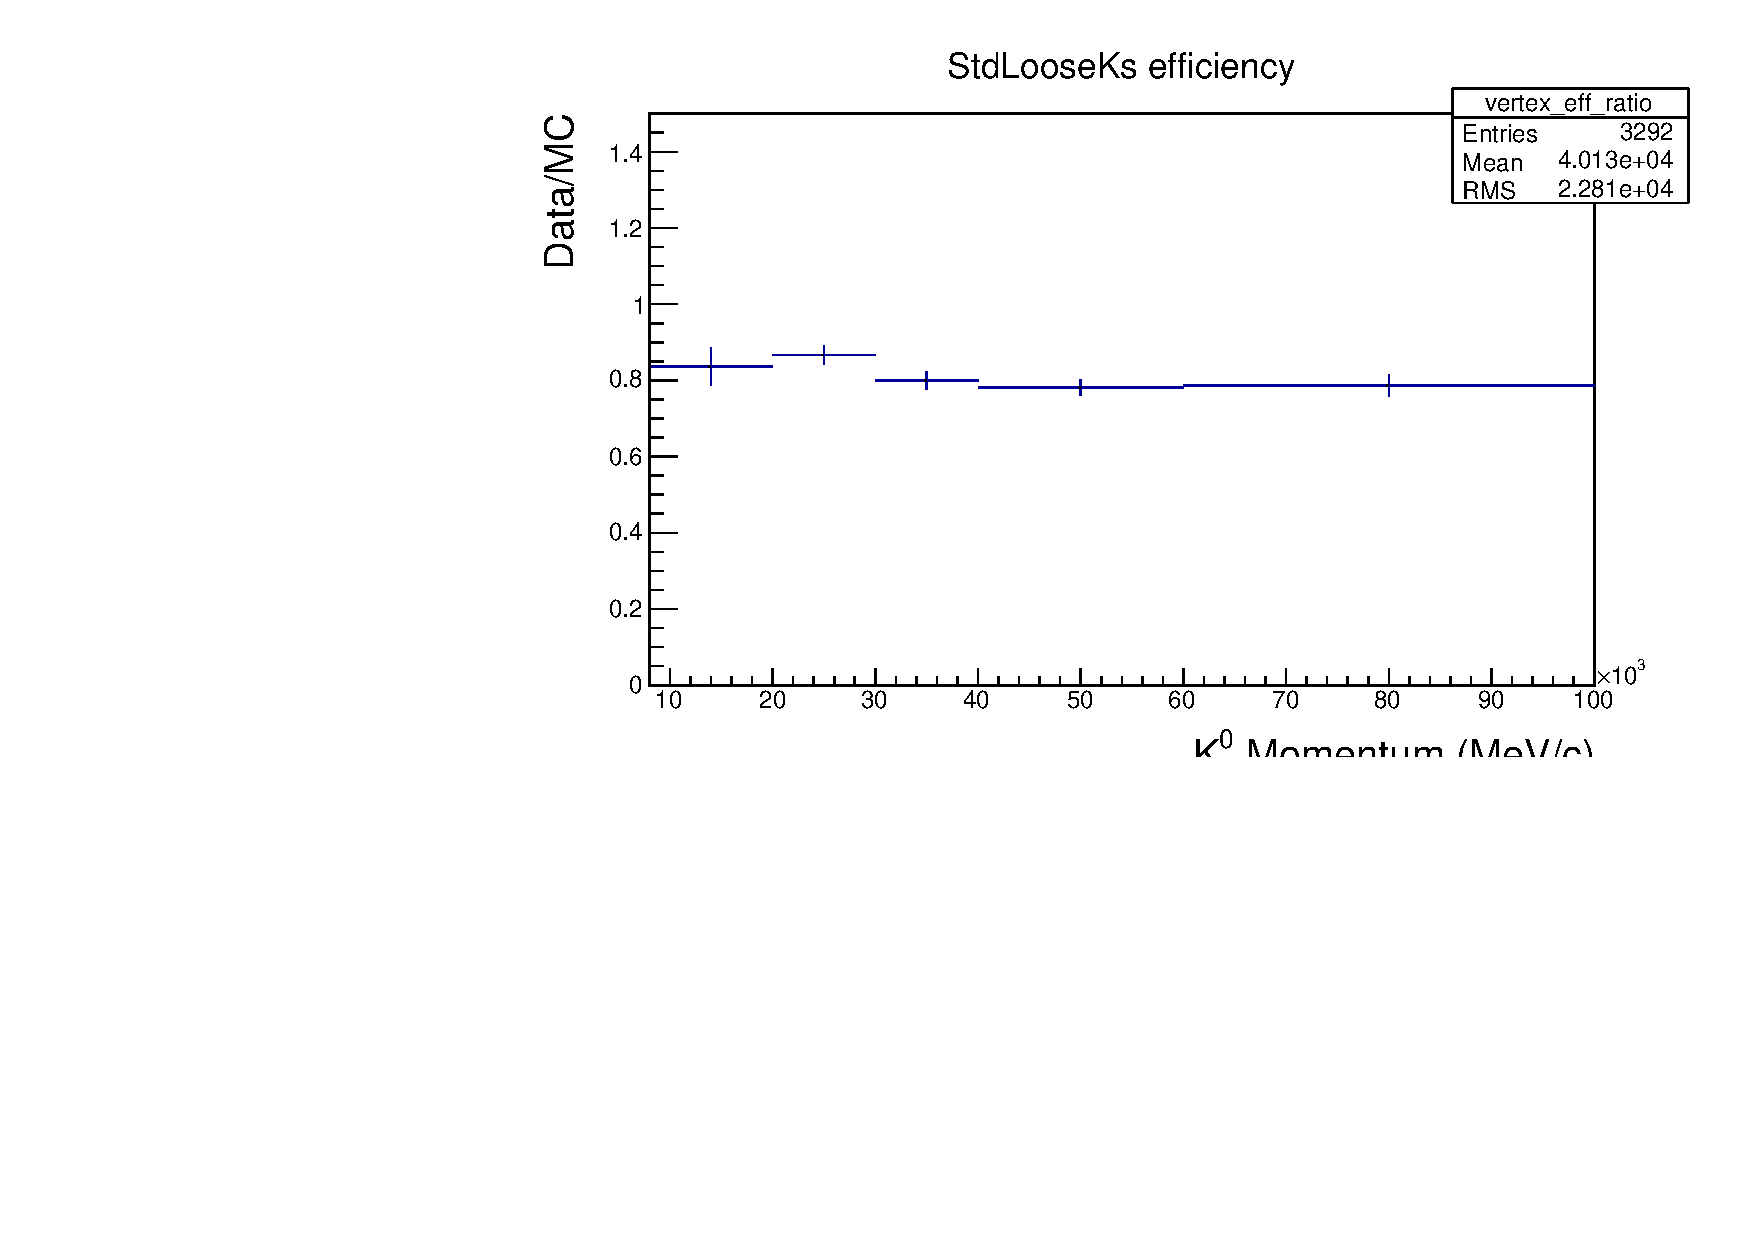
\includegraphics[width=0.6\textwidth]{Lmumu/figs/DDvtx_eff_POwen.pdf}
\caption{Ratio of reconstruction efficiency in Data and MC found using $K_S$ events~\cite{Blake:1631348}.}
\label{KS_vtxeff}
\end{figure}

This effect is dealt with in two steps. Firstly, the analysis separately for downstream and long candidates.
Since efficiencies are also calculated separately, the effect should mostly cancel in the ratio between the
rare and resonant channels. In a second step a systematic uncertainty is assigned for down-down events only.
To do this the simulation is re-weighed by the efficiency ratio between data and simulation
found for $K_S$ as a function of momentum and shown in Fig.~\ref{KS_vtxeff}. Then corrected and uncorrected
efficiencies are compared and the full difference is taken as systematic uncertainty. Dependencies due to
the different momentum distributions of \Lz and \KS are assumed to be negligible since 
the discrepancy shows little dependence on momentum. This results in an extra 0.4\% systematic at low \qsq
and 1.2 \% at high \qsq, only for downstream candidates.

\subsection{Data-simulation discrepancies}

The simulation used to extract efficiency is re-weighted as described in sec.\ref{sec:kinWeight}.
The influence on this procedure on the efficiencies was checked by comparing values obtained with
and without re-weighting. The effect is negligible with respect to other systematics considered.
%After the kinematical re-weighting there could still be some data-simulation discrepancies.
%In particular the PID variables, used in the Neural Networks, are not perfectly described in the MC.
%We checked if this could be a source of systematics by comparing sideband subtracted data Monte Carlo re-weighted for the
%\Lb kinematics and extracting a further weight to match the PID variable.
%Figure \ref{fig:PIDmysys} shows the difference between the efficiency calculated with and without the further PID weight.
%In all \qsq bins the difference is always compativle with zero within one sigma and therefore we do not add any further systematic
%due to the PIDmu variable modelling.

%\begin{figure}
%\centering
%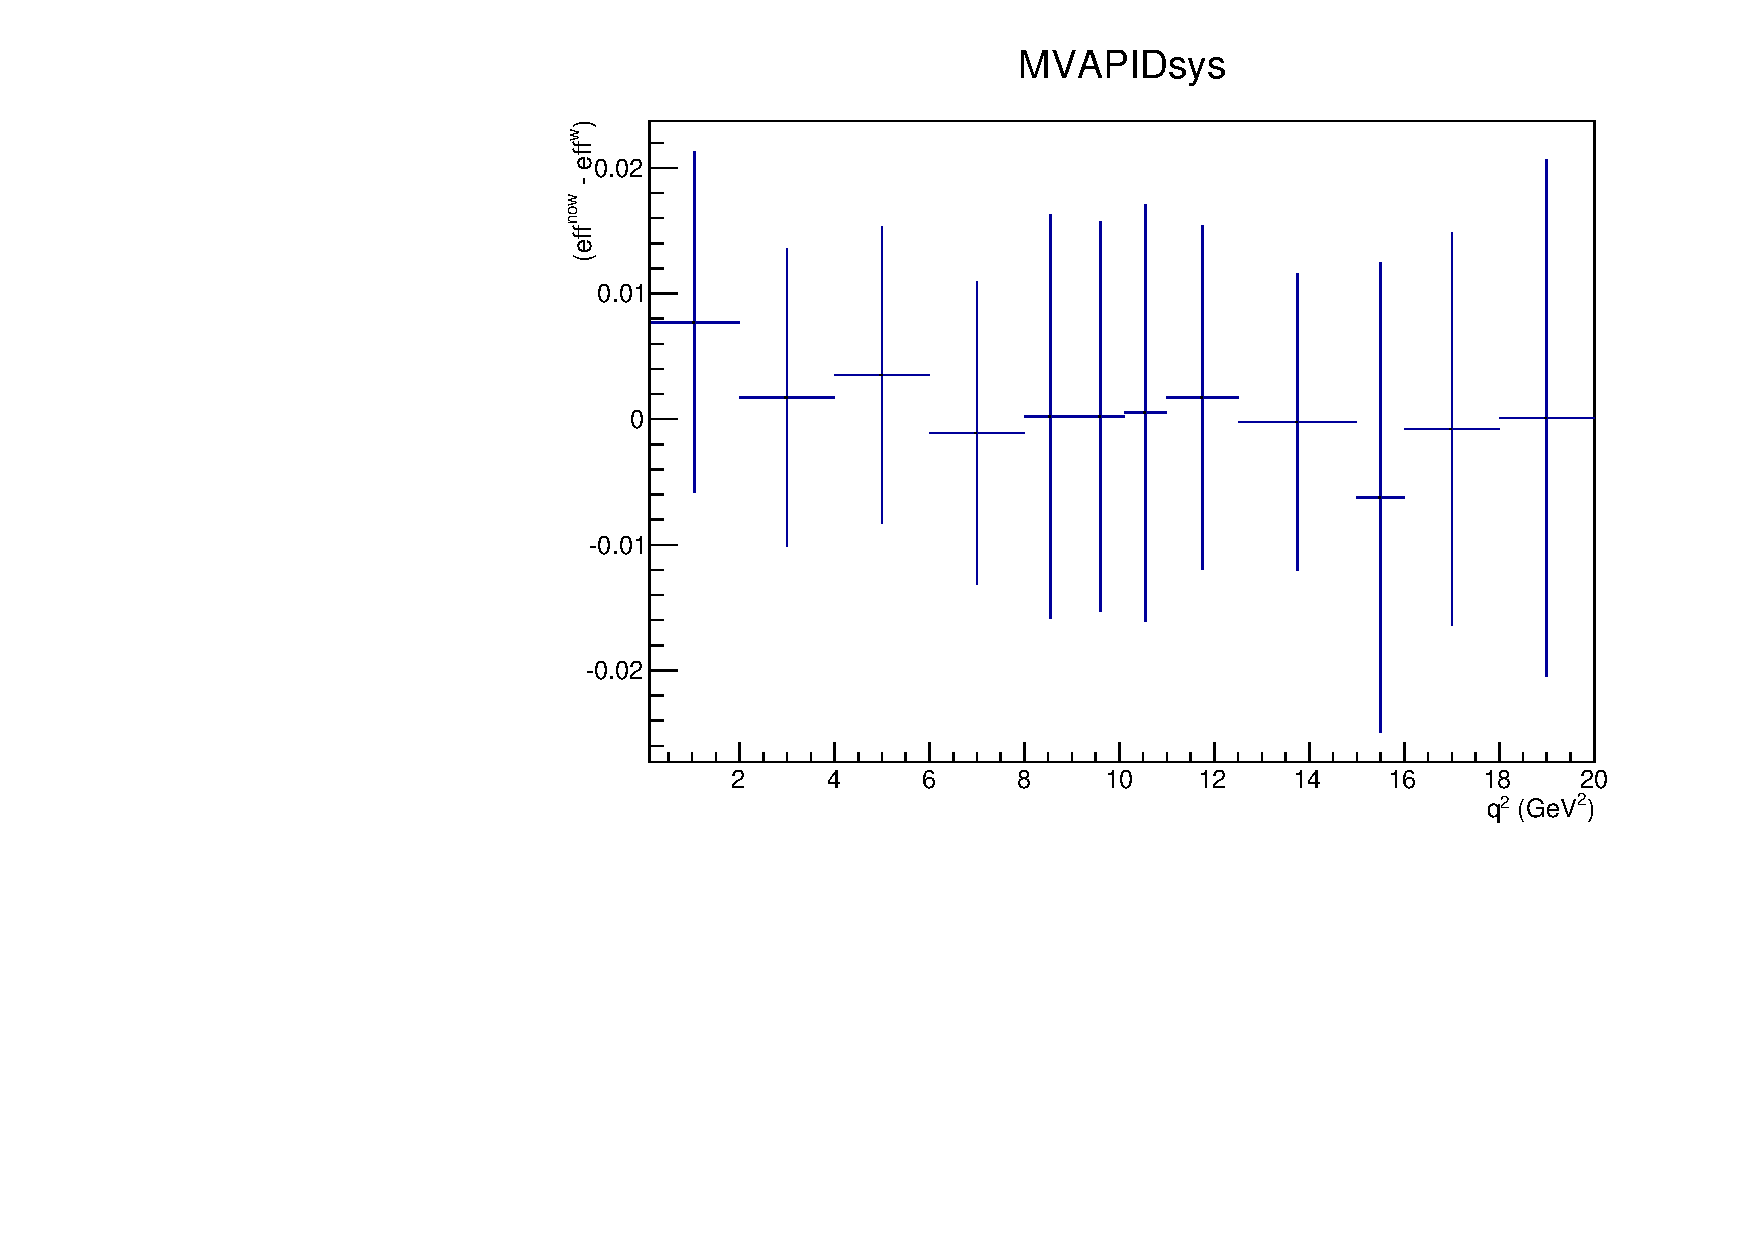
\includegraphics[width=0.6\textwidth]{Lmumu/figs/PIDmu_sys.pdf}
%\caption{Difference between the efficiency calculated with and without the weight to match the PIDmu distributions
%in data and MC as a function of \qsq.}
%\label{fig:PIDmysys}
%\end{figure}









